\documentclass[letterpaper,12pt]{article}
\usepackage{tabularx} % extra features for tabular environment
\usepackage{amsmath}  % improve math presentation
\usepackage{float}
\usepackage{pdfpages}

\usepackage{multicol}
\usepackage{graphicx} % takes care of graphic including machinery
\graphicspath{ {./figures/} }
%\usepackage[margin=1in,letterpaper]{geometry} % decreases margins
%\usepackage{cite} % takes care of citations
\usepackage[final]{hyperref} % adds hyper links inside the generated pdf file
\hypersetup{
	colorlinks=true,       % false: boxed links; true: colored links
	linkcolor=blue,        % color of internal links
	citecolor=blue,        % color of links to bibliography
	filecolor=magenta,     % color of file links
	urlcolor =blue         
}
\usepackage[margin = 1in,headsep=0.5cm,headheight=2cm,letterpaper]{geometry} 

\usepackage{fancyhdr}
\pagestyle{fancy}
\lhead{Student 1 : Ahmet Akman 2442366 \\ Student 2: Yusuf Toprak Yıldıran 2444149 \\ Assistant: Onur Selim Kılıç}
\rhead{Date: \today \\ Group: Wednesday Morning - 5} 
%\cfoot{center of the footer!}
\renewcommand{\headrulewidth}{0.1pt}



\begin{document}
\thispagestyle{empty}

\title{Spring 2022 EE214 Experiment 5  \protect\\ Bipolar Junction Transistor Characteristics}
\author{Ahmet Akman 2442366 \protect\\ Yusuf Toprak Yıldıran 2444149 \protect\\ Assistant: Onur Selim Kılıç}
\date{\today}
\maketitle
\tableofcontents
%\begin{abstract}
%abstract
%\end{abstract}
\section{Introduction}
In this experiment, using the diode test method, checking if the BJT transistor is NPN or PNP will be applied, and setting up a correct test environment with BenchVue will be learned. Finally, input-output characteristics of both NPN and PNP bipolar junction transistors will be investigated.

\section{Experimental Results and Discussion}
The results of the experiment are discussed in the following steps.
%
\subsection{Step 1}
In this step of the experiment, it is investigated whether the transistors in the lab are working or not. To check, the diode test feature of the digital multimeter is used. The multimeter gives a buzz when the PN junction is connected in the forward direction. To illustrate what is inside a transistor, a representative figure for an NPN transistor is given in Figure 1.

\begin{figure}[H]
    \centering
    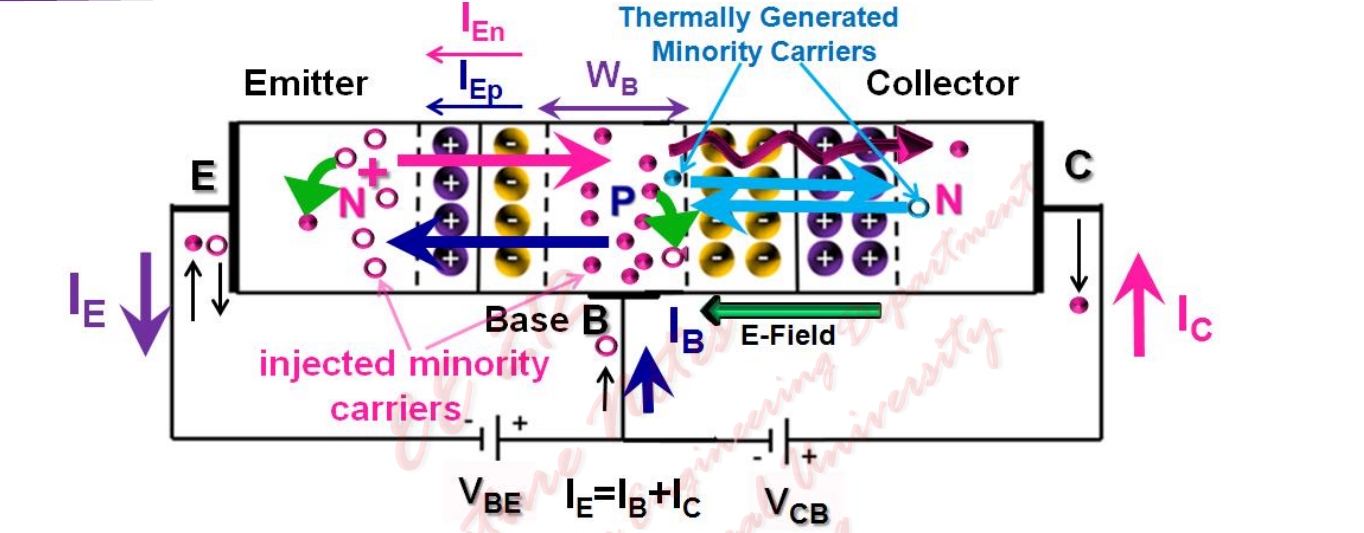
\includegraphics[width = 0.75\textwidth]{bjt.png}
    \caption{NPN BJT Sketch}
\end{figure} 
So, for NPN BJT, the multimeter buzzes for base-emitter and base-collector directions. Similarly, for PNP BJT, the multimeter buzz for emitter-base and collector-base directions.

\subsection{Step 2}
In this part of the experiment,\(I_B\) vs \( V_{BE}\) characteristics of the NPN type BJT transitor is obtained.

\begin{figure}[H]
    \centering
    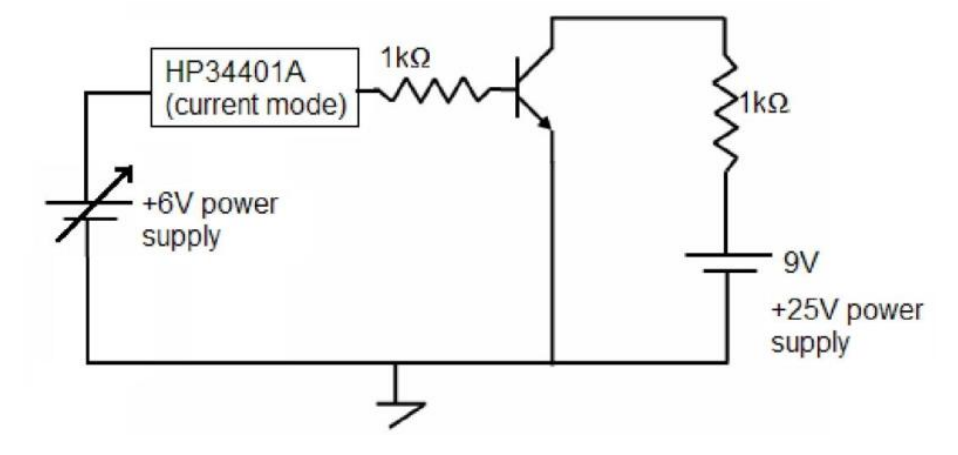
\includegraphics[width = 0.75\textwidth]{step2.png}
    \caption{Circuit schematic for the step 2}
\end{figure} 

After setting up the following common-emitter circuit in Figure 2, a test environment named BenchVue Test Flow is designed by following the steps below:
\begin{itemize}
    \item i. Initialize and launch the devices.
    Launch the program BenchVue, which you can find on the desktop.
    In this experiment, we will use the digital multimeter and DC power supply. Firstly,
    turn on these devices manually. Then, launch the device “DMM” (Digital Multimeter)
    and “Power Supply” by double-clicking on their icons, which you can find in the lower
    right corner of the BenchVue screen. This action will activate the remote mode on these
    devices. In remote mode, control of these devices is completely transferred to the
    BenchVue program, and you can no longer control the devices using their buttons.
    Observe that the launched devices are now at the lower-left corner of the screen. You
    can reach the control panel of the devices by double-clicking on them. Take a look at
    the control panel of both devices.
    \item ii. Construct the test flow. Test flow is a sequence of commands through which we can control
    the settings of devices and take measurements from the devices.
    Open the control panel of the Power supply. You will see three channels, each of which
    has a separate panel. +6V, +25V, and -25V outputs of the DC power supply are
    referred to as the first, second, and third channels, respectively.
    The output state of these channels is at the upper right corner of the panel belonging to
    each channel, on which either “On” or “Off” is written. As a first step, we need to switch
    on the output states of the channels that we will use. In this experiment, we will use
    +6V (CH1) and +25V (CH2) outputs of the DC power supply. Click on the orange box
    enclosing the output states of these channels and drag them, respectively, into the test
    flow on the right-hand side of the screen. Choose “Set”, and choose “On”.
    Click and drag the orange box enclosing “Voltage Setting” of +25V output (CH2) into
    the test flow. Choose “Set”. Enter 9V into the box.
    Click and drag the orange box enclosing “Voltage Setting” of +6V output (CH1) into
    the test flow. Choose “Sweep”. Enter the values in order for this source to sweep from
    100 mV to 2V by 200mV increments. Next, we will fill in the actions that are needed
    in each increment inside this sweep box.
    For each value of this source, we will take measurements. Always, we need to put some delay before taking measurements. Inside the sweep box, place a “Delay” block of 1
    second. You can find it in “More Blocks” > “Basic Blocks”.
    We will obtain the base current from the reading of the multimeter. Since we want to
    use that in a plot, we should assign that reading to a variable. Create a variable named
    “Ib” from “More Blocks” > “Variables” > “Create Variable”.
    In “More Blocks” > “Variables”, drag the label “Set” into the test flow. Then, drag the
    purple label for “Ib” to the left of “=” sign.
    Open the control panel of the digital multimeter (DMM). Set the “Measurement” as
    “DC Current”. Now the DMM works as an ammeter and please be sure that you have
    connected it into your circuit in series.
    You can see the readout panel at the right side of the control panel of DMM. Click and
    drag the readout box into the right of the “=” sign, so that the current reading is assigned
    to the variable “Ib”.
    We will calculate the base-emitter voltage and assign it into a variable named “Vbe”.
    Create this variable and prepare the assignment procedure just as you did for “Ib” in previous step. (Repeat the procedure)
    “Vbe” is equal to the voltage drop across the base resistor subtracted from the voltage value
    of 6V power supply. Using subtraction and multiplication boxes, fill in the boxes on the right. 
    Assignment of “Vbe” was the last step that will be done inside the sweep. Set the output
    states as “Off” outside the sweep box which will conclude the flow.
    In the end, the test flow should look like Figure x.
    \item iii. By using a multimeter as an ammeter(HP34401A), click on the run button. Then, by selecting X-Y chart \(I_B vs. B_{BE}\) plot is obtained as in Figure 3.
\end{itemize}

\begin{figure}[H]
    \centering
    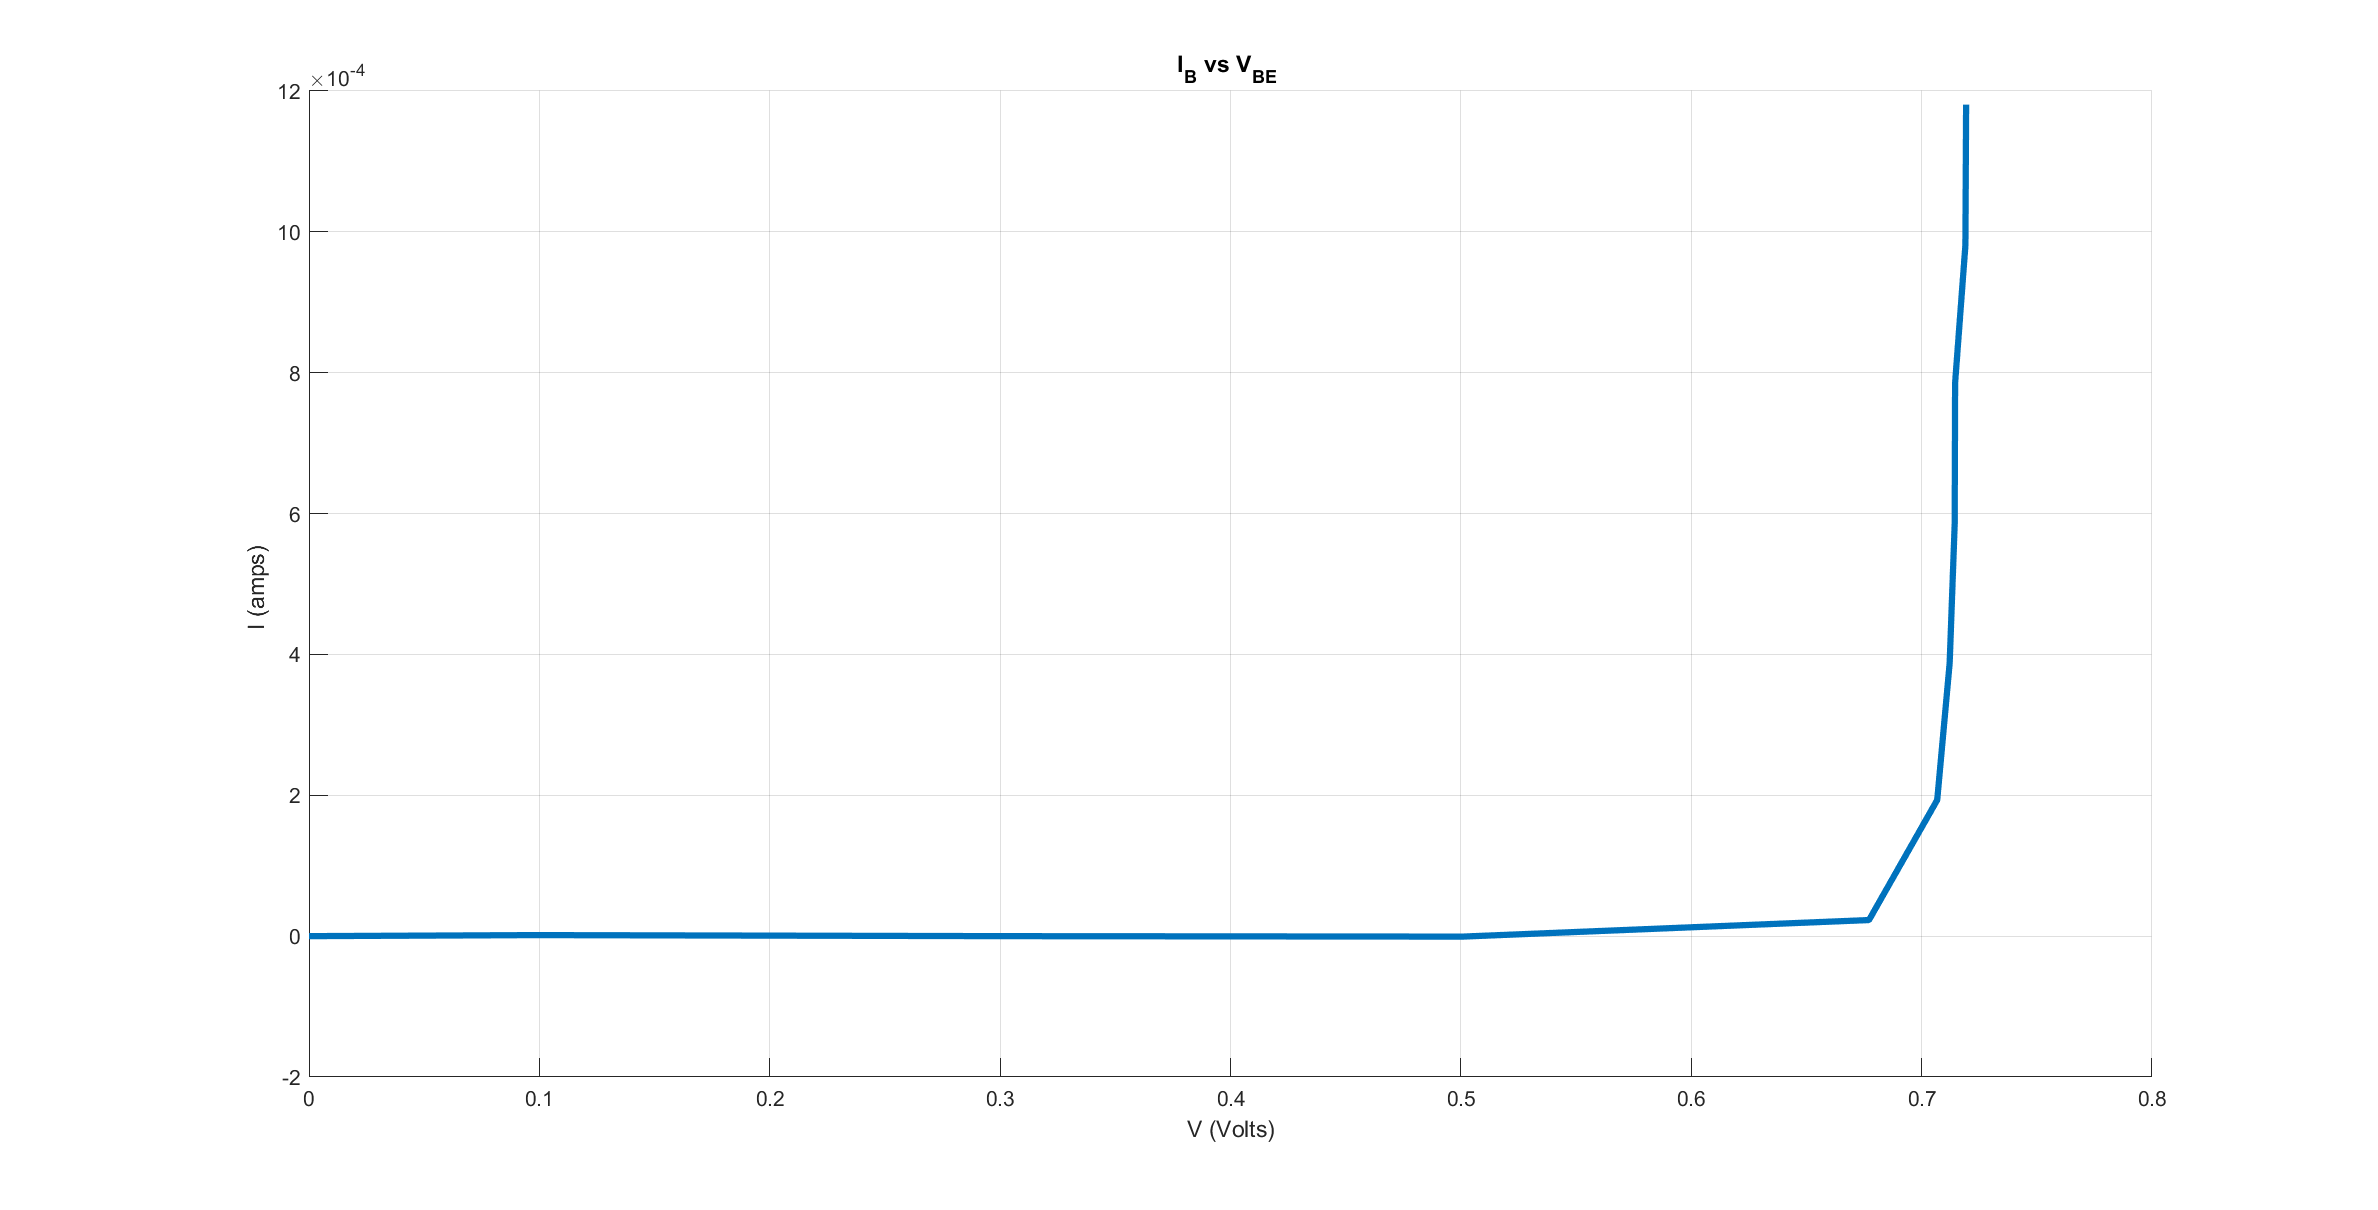
\includegraphics[width = 0.75\textwidth]{2_1.png}
    \caption{Plot obtained for the step 2}
\end{figure} 

Afterward, the designed circuit is tested in this environment, and as seen in Figure 3, the plot is like the i-v characteristics of a diode with an opening voltage is around 600mV since Vbe is a PN junction. If it is commented on it, it can be said that after \( V_{BE}\) is passed, 600mV current starts to flow, so \( V_{BE}\) can be called opening voltage.    

\subsection{Step 3}

\subsubsection{a)} 
In this part, the circuit in Figure 4 is set, and \(I_C\) vs. \(V_{CB}\) characteristics of the NPN transistor are investigated by again setting up a proper test environment using BenchVue. 
\begin{figure}[H]
    \centering
    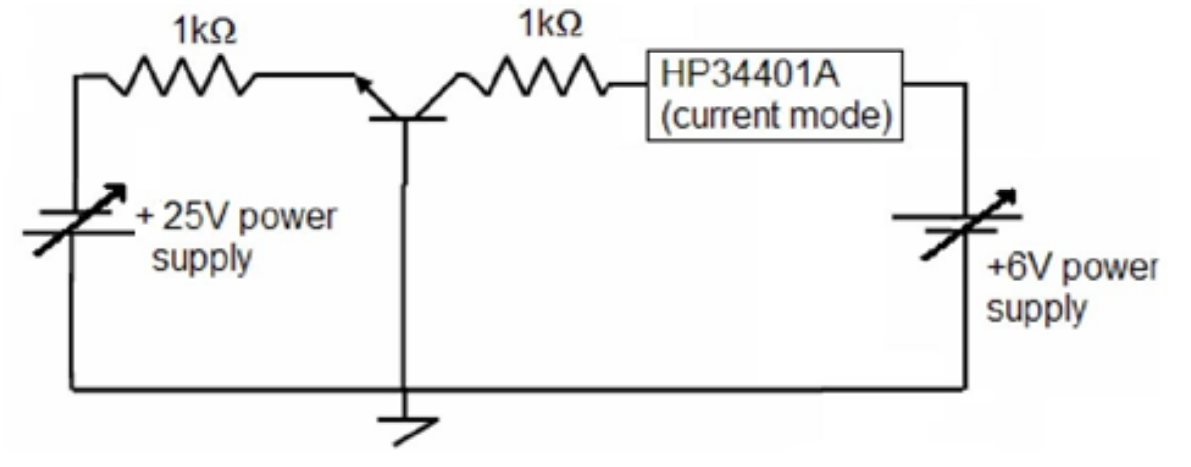
\includegraphics[width = 0.75\textwidth]{step3.png}
    \caption{Circuit schematic for the step 3 part a}
\end{figure} 

Since there are two voltage sources to be swept, first +25V channel is swept from 4V to 6V with steps of 1V, and then another source(6V channel) is swept inside of the previous swept block from 1V to 6V with 0.5V steps.  
Afterward, the following plot is obtained in Figure 5. The reason why we observed \(I_C\) current while \(V_{CB}\) is negative is because \(V_{BC}\) is positive and allows current to flow from base to collector.

\begin{figure}[H]
    \centering
    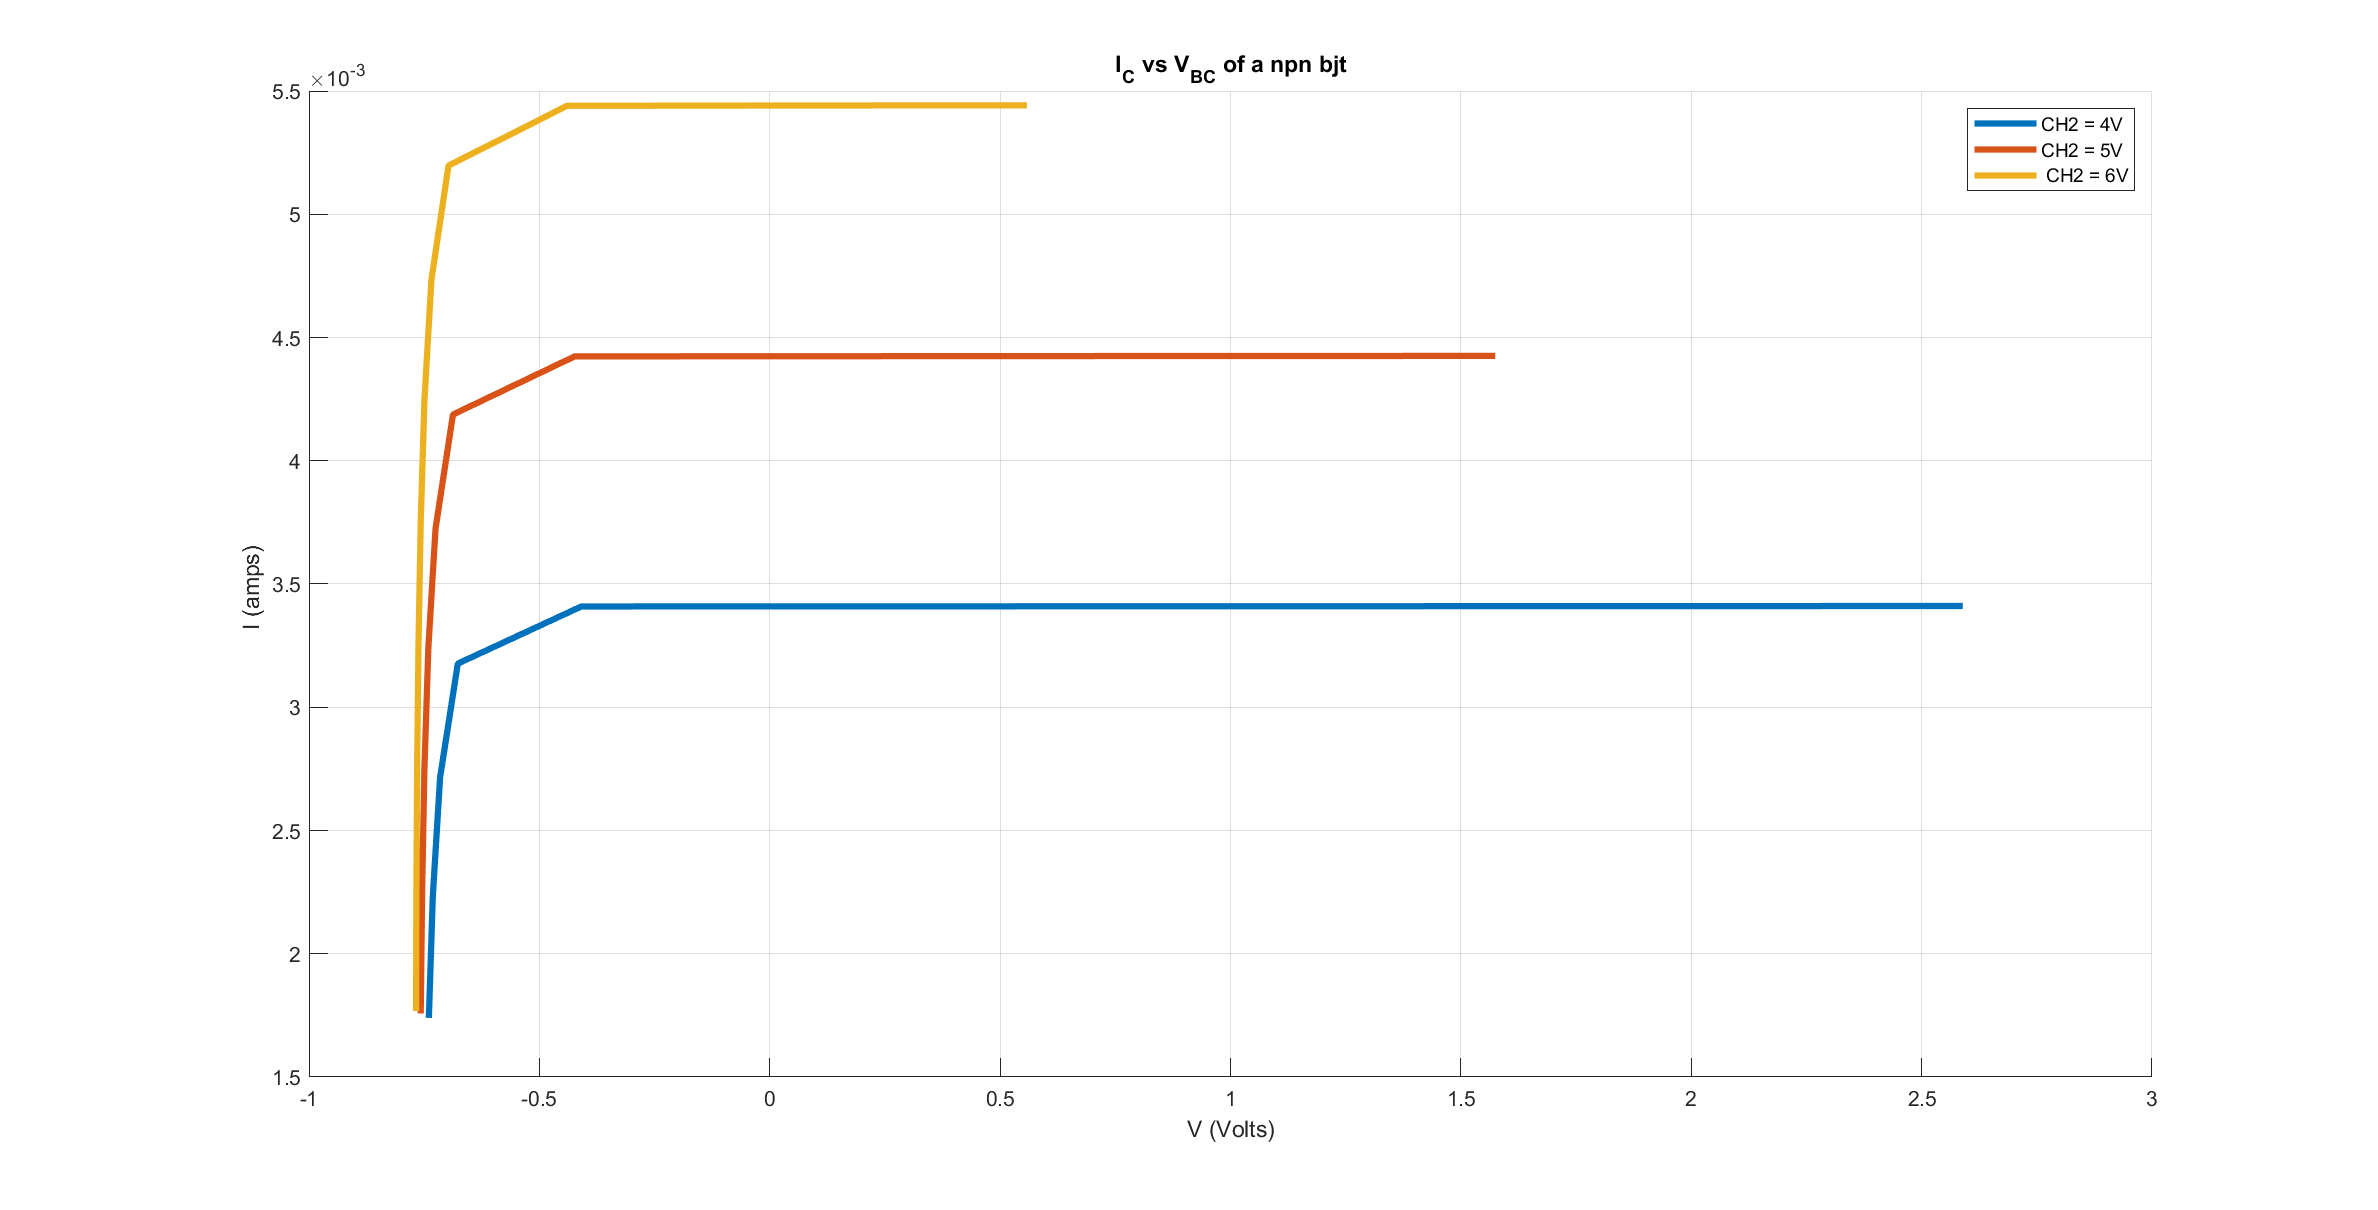
\includegraphics[width = 0.75\textwidth]{3_1.png}
    \caption{Plot obtained for the step 3 part a}
    \end{figure} 
\subsubsection{b)}
For this step, the circuit in Figure 4 is set in order to observe \(I_C\) vs. \(V_{BC}\) characteristics of the PNP transistor(C557B) with a suitable test environment as in the previous part in BenchVue. To be able to run the circuit in forward bias B-E junction and use the same environment settings as the previous part in this part, voltage sources should be reverse connected for the Figure 4. Then, step 3, part a) is repeated for this circuit, and Figure 6 is obtained. Because of the diode model, the fact that the direction definition of \(I_C\) is changed is noted. 
\begin{figure}[H]
    \centering
    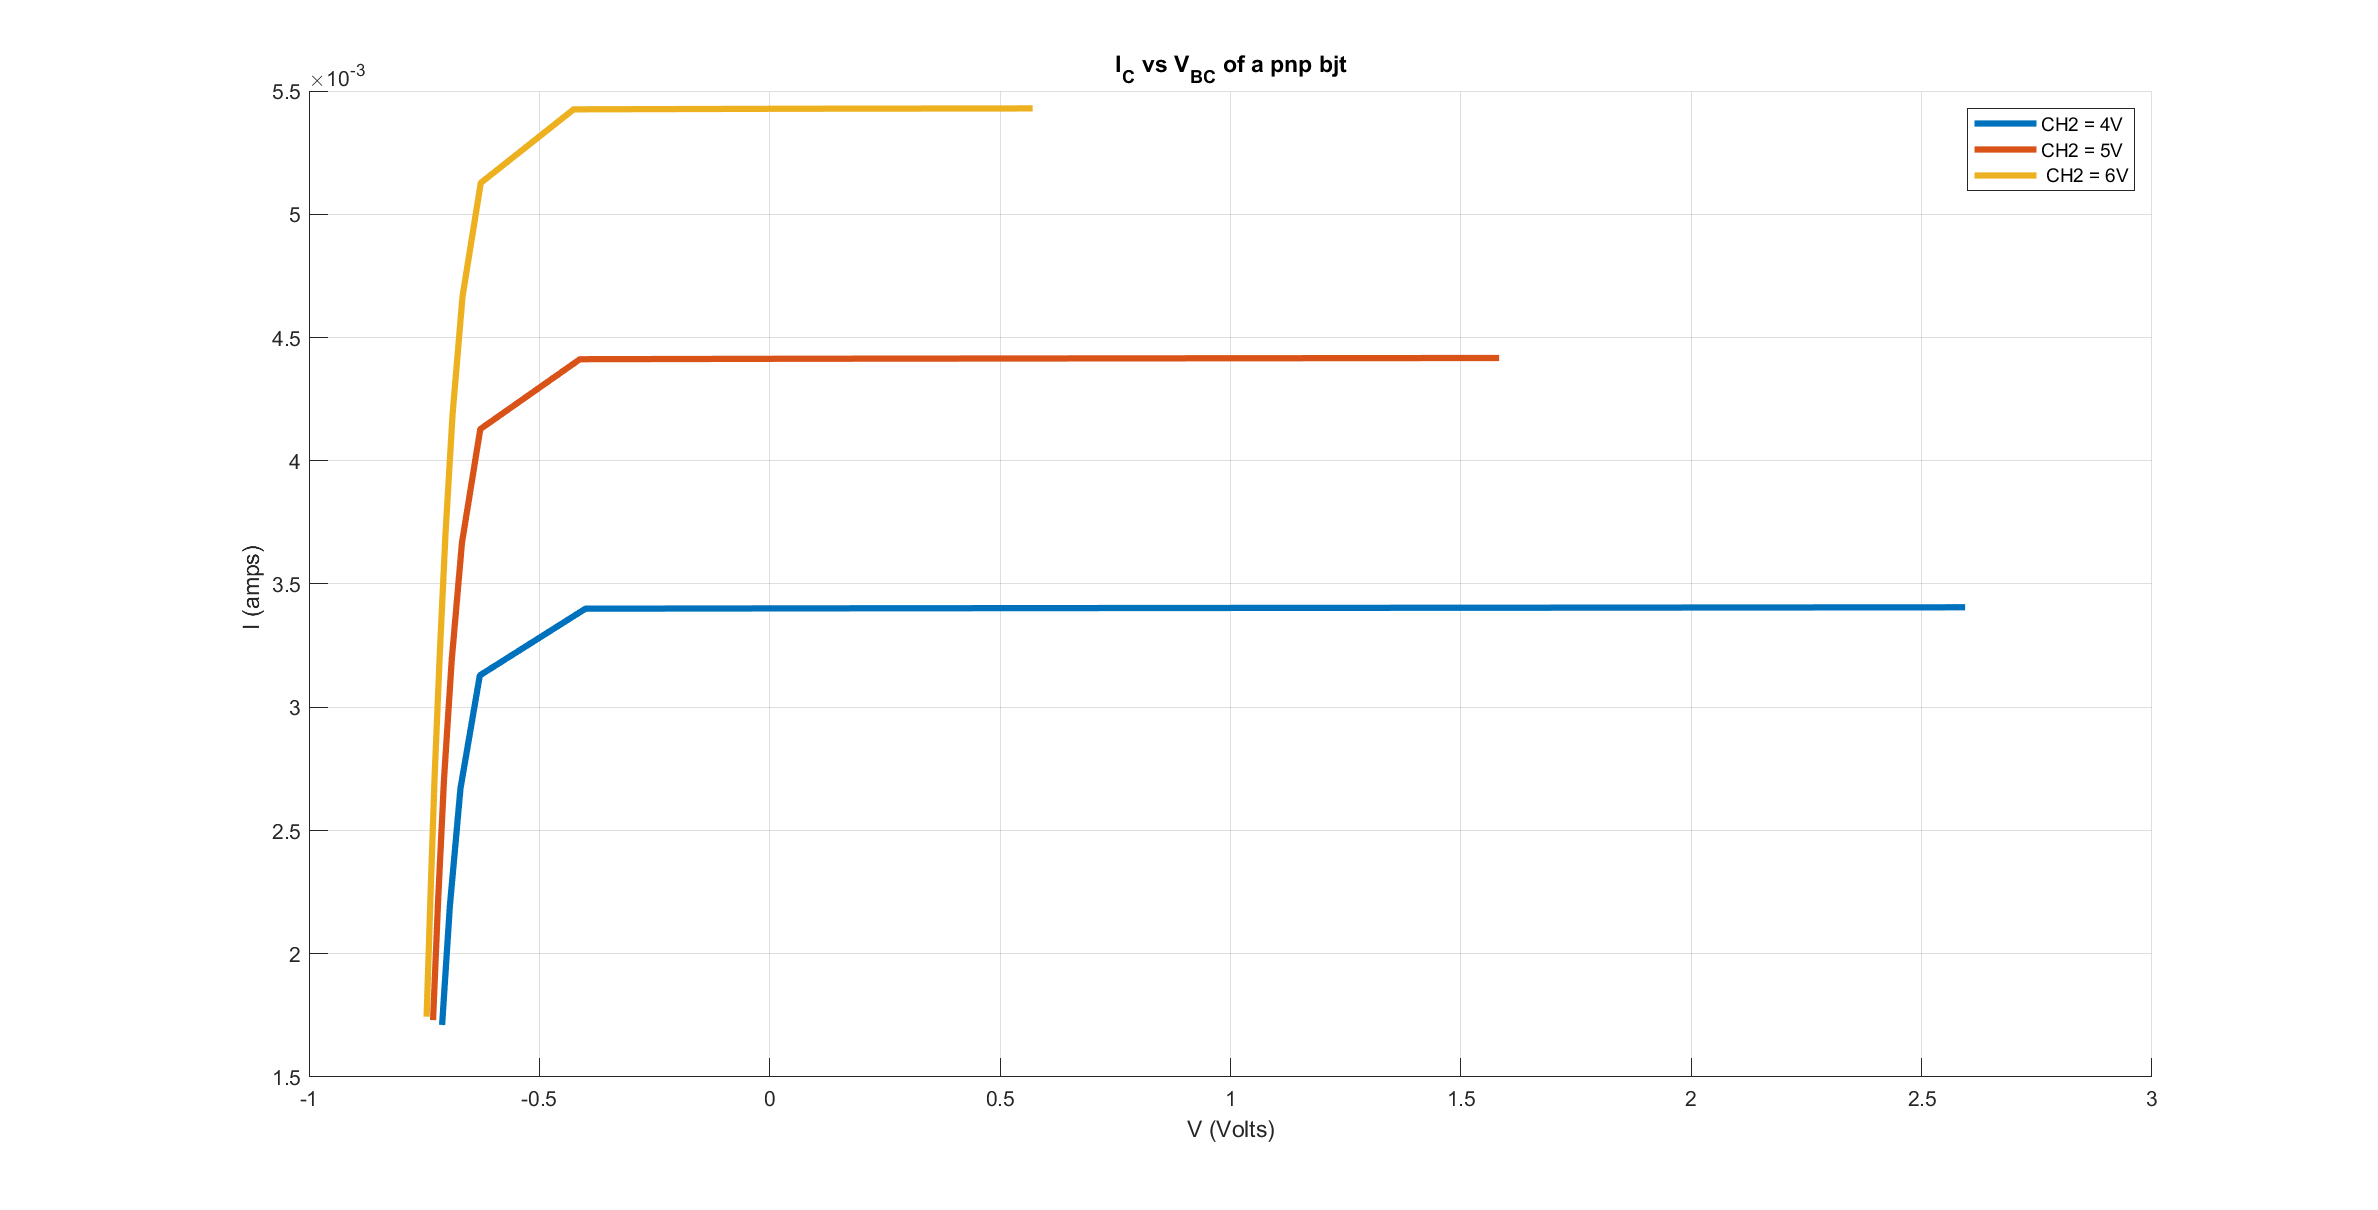
\includegraphics[width = 0.75\textwidth]{3_2.png}
    \caption{Plot obtained for the step 3 part b}
    \end{figure} 
\subsection{Step 4}
In this step, the circuit in Figure 7 is set in order to observe \(I_C\) vs. \(V_{CE}\) characteristics of the NPN transistor(C547B) with a proper test environment as done in previous steps in BenchVue. 

\begin{figure}[H]
    \centering
    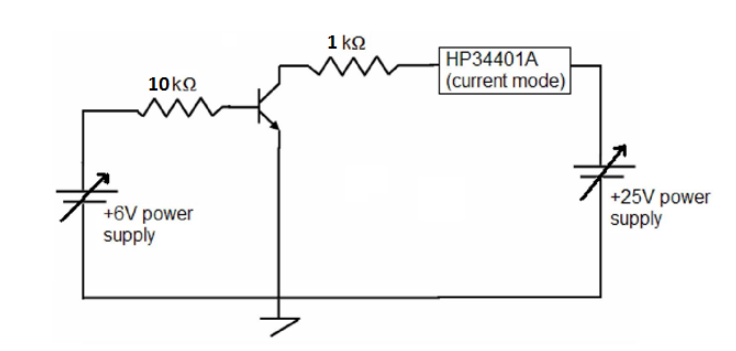
\includegraphics[width = 0.75\textwidth]{step4.png}
    \caption{Circuit schematic for the step 4}
    \end{figure} 
\subsection{Step 4}
So as a result the plot given in Figure 8 is obtained


\begin{figure}[H]
    \centering
    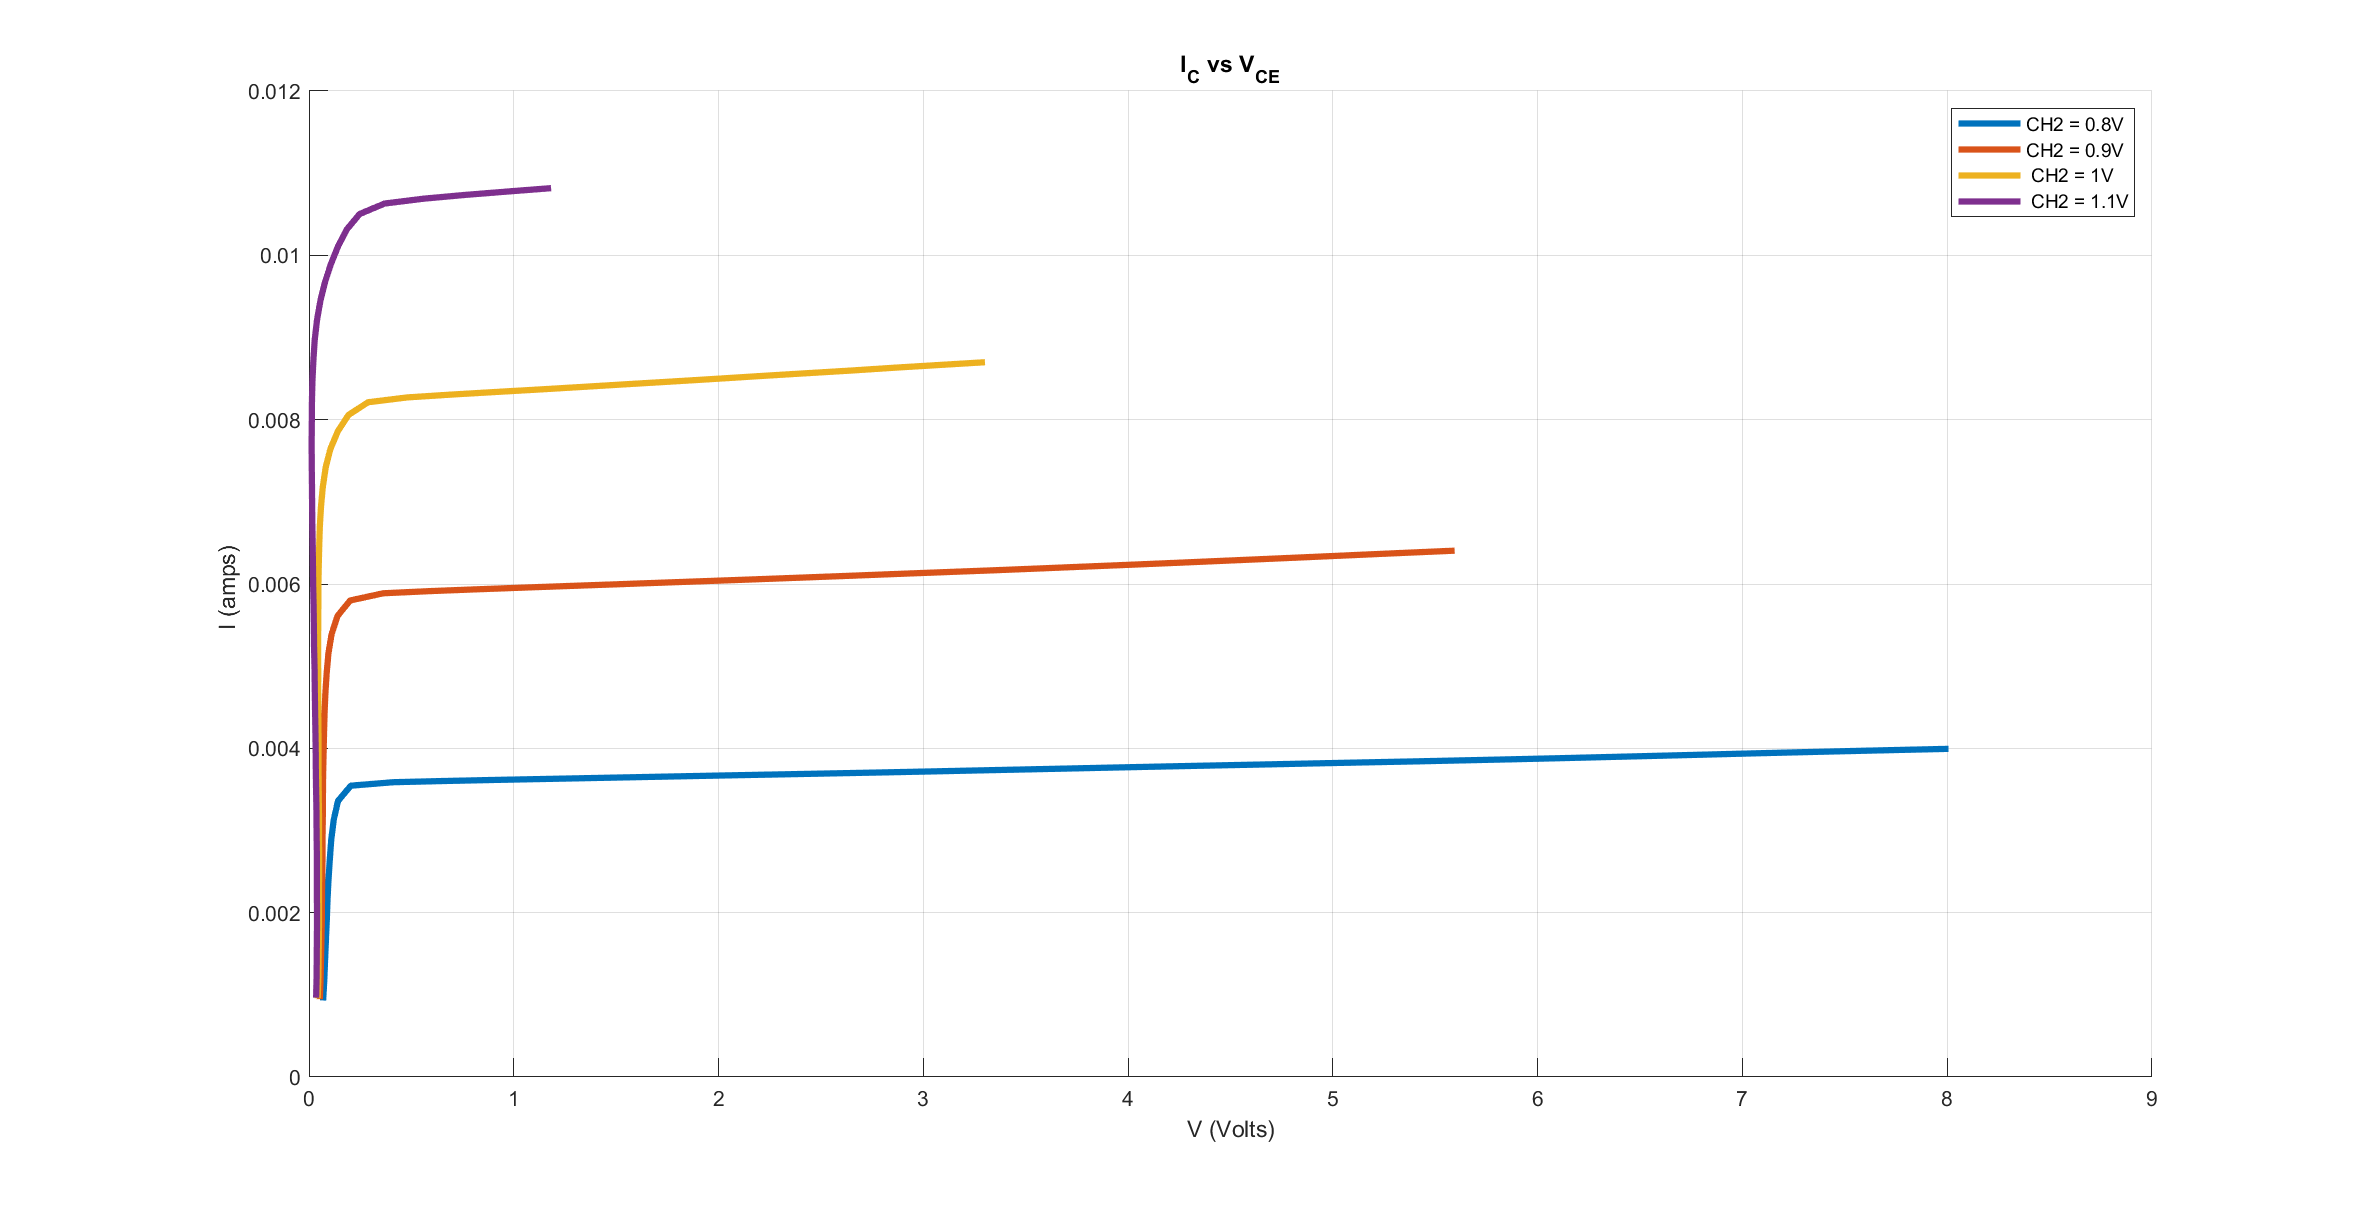
\includegraphics[width = 0.75\textwidth]{4_1.png}
    \caption{Plot obtained for the step 4}
    \end{figure} 

It can be said that there are slopes for the forward active regions of the transistor. This is called the early effect. The early effect is stemmed from the fact that effective base width changes with the applied base-collector voltage. The early voltage is defined and can be calculated with the interpolation of the forward region lines and finding the voltage in which the interpolated line intersects with the x-axis. This technique is illustrated in Figure 8 as well. 

\section{Conclusion}
In this experiment, using the diode test method, checking if BJT transistor is NPN or PNP will is applied, and setting up a correct test environment with BenchVue is learned. Afterward, input-output characteristics of both NPN and PNP bipolar junction transistors are investigated.

\section*{Appendix A}
\begin{itemize}
    \item PreLab Preparation 3 hours
    \item Experimental Work 2  hours
    \item Report Writing 8 hours
\end{itemize}
\section*{Appendix B}
In this experiment, since the values the students obtained in the lab is quite close to the data provided by the lab assistants, it is preffered to use the data obtained by the students.

\end{document}

%%%%%%%%%%%%%%%%%%%%%%   EXAMPLE TABLE   %%%%%%%%%%%%%%%%%%%%%%%%%%%%%%%%
\begin{table}[H]
\begin{center}
    \caption{Resistance reading by color code convention.}
    \vspace{2mm}
    \begin{tabular}{||c | c | c||} 
        \hline
        Color Order & Value & Tolerance \\ [0.5ex] 
        \hline\hline
        Brown / Black / Red / Gold & 1k\( \Omega \) & \( \% \) 5  \\ 
        \hline
        Yellow / Violet / Red / Gold & 4.7k\( \Omega \) & \( \% \) 5   \\
        \hline
        Brown / Grey / Orange / Gold & 18k\( \Omega \) & \( \% \) 5  \\ [1ex] 
        \hline
    \end{tabular}
\end{center}
\end{table}


%%%%%%%%%%%%%%%%%%%%%%   EXAMPLE IMAGE   %%%%%%%%%%%%%%%%%%%%%%%%%%%%%%%%
\begin{figure}[H]
\centering
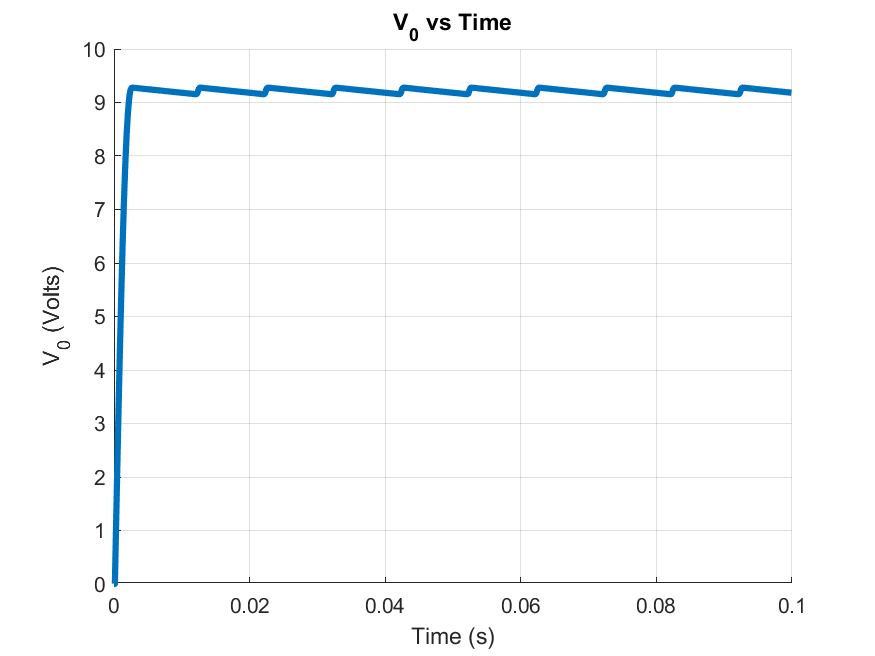
\includegraphics[width = 0.75\textwidth]{5.png}
\caption{Circuit schematic for the step 5}
\end{figure} 

%%%%%%%%%%%%%%%%%%%%%%   EXAMPLE IMAGE FROM PDF   %%%%%%%%%%%%%%%%%%%%%%%%%%%%%%%%
\begin{figure}[H] \centering{
	\includegraphics[scale=0.25]{2a_plot.pdf}}
	\caption{Experiment 2}
\end{figure}
%%%%%%%%%%%%%%%% Deneme Push